\documentclass[11pt,a4paper]{article}

\usepackage[T1]{fontenc}
\usepackage[utf8]{inputenc}
\usepackage[english]{babel}
\usepackage{lmodern}
\usepackage[margin=2.5cm]{geometry}
\usepackage{microtype}
\usepackage{graphicx}
\usepackage{float}
\usepackage[labelsep=period,font=small,labelfont=bf]{caption}
\usepackage{setspace}
\usepackage{booktabs}
\usepackage{tabularx}
\usepackage{array}
\usepackage{xcolor}
\usepackage{multicol}
\usepackage{listings}
\usepackage[hidelinks]{hyperref}

% Code listings
\lstset{language=C++, basicstyle=\ttfamily\footnotesize, keywordstyle=\bfseries,
  commentstyle=\itshape\color{black!60}, columns=fullflexible, keepspaces=true,
  frame=single, rulecolor=\color{black!30}, framesep=4pt, xleftmargin=6pt, xrightmargin=6pt,
  breaklines=true, showstringspaces=false, aboveskip=0.6em, belowskip=0.8em}

% Commit identifier linked to the GitHub repository
\newcommand{\commit}[1]{\href{https://github.com/riyyan-ahmed/TSP-Solver-Project/commit/#1}{\texttt{#1}}}
% Left-aligned paragraph column for tables
\newcolumntype{L}[1]{>{\raggedright\arraybackslash}p{#1}}
\newcolumntype{Y}{>{\raggedright\arraybackslash}X}

\setstretch{1.08}
\frenchspacing
\renewcommand{\topfraction}{0.85}
\renewcommand{\bottomfraction}{0.6}
\renewcommand{\textfraction}{0.1}
\renewcommand{\floatpagefraction}{0.8}
\setcounter{totalnumber}{4}
\setlength{\parindent}{1.2em}
\setlength{\parskip}{0.3em}
\setlength{\emergencystretch}{2em}

\title{Solving the Travelling Salesman Problem\\[0.3em]\large Design and Development Report}
\author{Riyyan \textsc{Ahmed} \and Salaheddine \textsc{Moustafid}}
\date{M1 AI, Universit\'e Grenoble Alpes\\
Mid-term checkpoint, 18 October 2026\\[0.4em]
\small Repository: \url{https://github.com/riyyan-ahmed/TSP-Solver-Project} (branch \texttt{riyyan-feature})}

\begin{document}
\maketitle

\begin{abstract}
\noindent
This report describes the development of a C++ solver for the metric Travelling Salesman Problem. We cover the chronology of the work, the tools we relied on, the structure of the code and the reasons behind the main design choices. At the time of writing, the program reads both TSPLIB formats required by the specification, runs the trivial method and writes tours in the required format. A test suite of 92 cases covers the parser, the graph classes, the tour writer and the compiled executable.
The tours produced for the provided instances were checked with the course solution checker, which accepted them as valid (for example, the trivial tour of \texttt{gr17} has length 4722).
\end{abstract}

\section{Introduction}

The goal of the project~\cite{subject} is a program that reads a TSP instance, computes a Hamiltonian cycle and writes it to a file. The specification asks for a build script at the root of the project, a \texttt{TSPsolver} executable taking an instance path, an output path and an optional method name, and a \texttt{tests} executable. It also fixes the input formats, namely a list of planar coordinates and the lower triangle of a weight matrix, and the output format, a permutation list ended by $-1$ and \texttt{EOF}.

Because the grading puts half of its weight on design quality, we separated the program into small components with clear responsibilities. Instance representation, distance computation, parsing, validation of tours and output are each handled by their own class, and each is covered by tests.

This report covers the mid-term checkpoint, for which the program must support the trivial method only. The Held-Karp algorithm and a third method of our choice will be added for the final submission, on top of the same parser, graph and output classes.

\section{Team and organisation}\label{sec-team}

We split the work by component (Table~\ref{tab-team}) and agreed early on the shared interfaces, mainly the instance and parser classes, so that each of us could work without waiting for the other. Each member worked on his own feature branch, \texttt{riyyan-feature} and \texttt{salah\_feature}, created from \texttt{master}, and we discussed the design together whenever a change affected both parts. Before the checkpoint, \texttt{salah\_feature} was merged into \texttt{riyyan-feature}, which is the branch we submit.

\begin{table}[H]
\centering\small
\begin{tabularx}{\linewidth}{@{}l Y l@{}}
\toprule
Member & Main responsibilities & Git branch \\
\midrule
Riyyan Ahmed & Decision parser (header reading and choice of the data section), \texttt{TspInstance}, lower diagonal parser, trivial method, integration for the checkpoint & \texttt{riyyan-feature} \\
Salaheddine Moustafid & Command line (\texttt{main}), coordinate parser and \texttt{CoordinatesGraph}, build script, test suite, first draft of the report & \texttt{salah\_feature} \\
\bottomrule
\end{tabularx}
\caption{Division of the work.}
\label{tab-team}
\end{table}

\section{Development process}\label{sec-process}

\subsection{Timeline}

Table~\ref{tab-timeline} lists the main steps of the project. Each push to the repository is given with its commit identifier.

\begin{table}[H]
\centering\small
\begin{tabularx}{\linewidth}{@{}l l Y L{2.6cm}@{}}
\toprule
Date & Who & Work & Commit \\
\midrule
21 Sep & Both & Reading of the subject and of the TSPLIB format, study of the 15 instance files, instances generated with \texttt{instance\_generator.py}, background reading on the TSP & -- \\
23 Sep & Both & Division of the work (Table~\ref{tab-team}) & -- \\
27 Sep & Riyyan & First data structure: distance matrix stored as a \texttt{vector<vector<double>{}>} inside \texttt{TspInstance} & -- \\
30 Sep & Riyyan & First push from the local project to the remote repository: instances, subject and CMake template & \commit{877cfb6}, \commit{48d86db} \\
1 Oct & Riyyan & Decision parser, header reading and lower diagonal parser, empty files for the planned structure & \commit{30e5ed7} \\
2--9 Oct & Riyyan & Review of the first draft and redesign into graph classes (Section~\ref{sec-challenges}) & -- \\
10 Oct & Riyyan & Redesigned version: \texttt{Graph}, \texttt{MatrixGraph}, \texttt{TspInstance}, \texttt{TspParser}, \texttt{TrivialSolver} & \commit{e8f5266} \\
11 Oct & Salah & Ignore file, \texttt{.DS\_Store} files removed from version control & \commit{2fa466f} \\
12 Oct & Salah & Command line and parse, solve, write pipeline in \texttt{main}, build script restored & \commit{a43ce1c}, \commit{d9129fc} \\
12 Oct & Salah & \texttt{CoordinatesGraph}, Euclidean distance and coordinate parser & \commit{c9edac5}, \commit{33d98a7}, \commit{b280887} \\
14--15 Oct & Salah & Review against the specification, bug fixes, test suite (84 tests), first draft of the report & \commit{86d5ae0} \\
16 Oct & Riyyan & Checkpoint fixes: CMake, build script, command line, city ids starting at 0, README, documentation comments, 92 tests & \commit{4287595} \\
16 Oct & Riyyan & Editor settings removed from version control & \commit{14ceb99} \\
17 Oct & Riyyan & Tours of the 15 instances, validation with the course checker, figures & \commit{052319b} \\
17 Oct & Both & Report completed (written alongside the code throughout the project) & -- \\
\bottomrule
\end{tabularx}
\caption{Timeline of the project. Commit identifiers link to the repository.}
\label{tab-timeline}
\end{table}

\subsection{Setting up the project}

After dividing the work on 23 September, we started implementing the project locally, and on 30 September we made our first push to the remote repository. The project is based on the template provided with the course, which already separates headers, sources and tests. We kept this layout. On 1 October we wrote the first version of the parser together with the code for the lower triangular matrix format, and created the empty files for the remaining parts of the architecture so that the structure was fixed before any algorithm existed.

The TSPLIB header needed some care. The entries may come in any order, the separator may or may not be preceded by a space across the provided files, and some entries such as comments can contain a second separator inside the value. We therefore split each header line at the first separator only, trim both parts, and ignore the entries we do not need.

\subsection{Matrix instances and the first solver}

By 10 October the parser handled the lower triangular format and the trivial method existed. Two properties of the provided files caused most of the work in this phase. First, the matrix is not guaranteed to be laid out with one row per line, so we read it as a stream of integers and rebuild the rows from the dimension. Second, one instance (\texttt{dantzig42}) is followed by a display data section holding coordinates that are only meant for drawing. Since the parser otherwise rejects data after the matrix, this section has to be recognised explicitly. We skip it up to the closing keyword and still reject any other trailing data.

\subsection{Command line and coordinate instances}

On 12 October we wrote the command line handling and connected the parser, the solver and the writer in \texttt{main}, so that the complete pipeline ran for the trivial method on the matrix instances. The build script was briefly lost during a clean up, and we restored it the same night, which showed us how easy it is to break the one requirement that is checked first. We then added the coordinate format in three small steps, the graph class, the Euclidean distance and the parsing of the coordinate section.

Since nothing forces the lines of a coordinate file to be sorted, each city is stored at the position given by its identifier, and the identifiers are kept so that the tour file uses those of the input (Section~\ref{sec-parsing}).

\subsection{Review and tests}

On 14 October we reviewed the code against the specification and wrote the test suite. The review found several defects that our manual runs had not shown: the test files were ignored by Git, an out of range matrix index caused undefined behaviour, the coordinate parser accepted data after \texttt{EOF}, and the build did not produce \texttt{build/TSPsolver} (challenges 3 and 4 in Table~\ref{tab-challenges}). The most instructive one concerned the tour writer. It opened the output file, which empties it, before checking that the tour was valid, so a faulty solver would have erased a previous result. The check now runs before the file is opened, and a test verifies that an invalid tour leaves an existing file unchanged.

The points that the subject leaves open, such as the optional \texttt{EOF} keyword and the distance types of coordinate files, are discussed with our decisions in Section~\ref{sec-limits}.

\subsection{Main challenges}\label{sec-challenges}

Table~\ref{tab-challenges} summarises the five main challenges we met, with their cause, our solution and the commit in which each was fixed.

\begin{table}[tbp]
\centering\small
\begin{tabularx}{\linewidth}{@{}c L{2.5cm} Y Y L{1.8cm}@{}}
\toprule
\# & Challenge & Cause & Solution & Commit \\
\midrule
1 & First data structure did not hold up & One raw matrix inside \texttt{TspInstance}, circular include with \texttt{TspParser.hpp}, private fields only reachable by the parser, coordinates lost & Class hierarchy based on the graph lab: abstract \texttt{Graph}, \texttt{MatrixGraph}, \texttt{CoordinatesGraph}; \texttt{TspInstance} owns its graph and has getters & \commit{30e5ed7} $\rightarrow$ \commit{e8f5266} \\
\addlinespace
2 & Irregular instance files & \texttt{KEY: v} and \texttt{KEY : v}, values containing \texttt{:}, matrix wrapped over lines, \texttt{DISPLAY\_DATA\_SECTION} in \texttt{dantzig42}, no \texttt{EOF} in \texttt{pr1002} & Split on the first \texttt{:} and trim, weights read as a stream, display section skipped, \texttt{EOF} optional but data after it rejected & \commit{30e5ed7}, \commit{e8f5266}, \commit{86d5ae0} \\
\addlinespace
3 & Build not matching the specification & Executable named \texttt{main} in the wrong folder, tests not built, global \texttt{-Werror} breaking GoogleTest & Warnings as errors only on our targets, executable renamed \texttt{TSPsolver}, build into \texttt{./build} with the tests & \commit{e8f5266}, \commit{86d5ae0} \\
\addlinespace
4 & Bugs found only by the tests & \texttt{tests/} ignored by Git, out of range matrix index (undefined behaviour), invalid tour emptied the output file & Ignore rule removed, index checks with exceptions, tour validated before the file is opened, regression tests & \commit{86d5ae0} \\
\addlinespace
5 & Generated instances rejected & \texttt{instance\_generator.py} numbers cities from 0, the parser required ids from 1 & Ids may start at 0 or 1, cities stored by id, tests for both cases & \commit{4287595} \\
\bottomrule
\end{tabularx}
\caption{Main challenges, their cause, our solution and the commit where it was fixed.}
\label{tab-challenges}
\end{table}

The two hardest challenges were the first and the third of Table~\ref{tab-challenges}. Replacing our first data structure meant rewriting the instance class and part of the parser after the first push, but it paid off: the coordinate format was later added in three small commits without touching the existing code. The build problems were harder to notice, because the program worked on our machines while the exact commands of the specification failed; since then we check the build from a clean copy of the repository, as a grader would.

\section{Tools and libraries}

The solver is written in C++20 and uses only the standard library. The data structures needed here (vectors, strings, streams and smart pointers) are all available there, and avoiding other dependencies keeps the build simple on the machines used for grading. The project is built with CMake, and our own targets are compiled with warnings treated as errors, which keeps the code free of unused variables and sign comparison problems.

The tests use GoogleTest~\cite{gtest}, which CMake downloads when the project is configured. It is the only external component, and only the test executable uses it. We chose it because it supports parameterised tests, which let us run the same checks on every provided instance.

Table~\ref{tab-tools} lists all the tools we used.

\begin{table}[htbp]
\centering\small
\begin{tabularx}{\linewidth}{@{}L{4.2cm} Y@{}}
\toprule
Tool & Used for \\
\midrule
C++20 and its standard library & All the code of the solver, without other dependencies \\
CMake & Building the library, \texttt{TSPsolver} and \texttt{tests} \\
GoogleTest & Unit tests and tests of the executable (downloaded by CMake) \\
Git and GitHub & Version control, one feature branch per member \\
Visual Studio Code on macOS & Writing and debugging the code \\
\texttt{instance\_generator.py} & Random instances of a chosen size, beyond the 15 provided files (provided by the course) \\
Course solution checker & Validation of our tour files, as a Moodle VPL activity and as the script \texttt{tsp\_check.py} (university network or VPN) \\
Python~3 & Running the generator, the checker script and a small timing script \\
\LaTeX{} & Writing and compiling this report \\
\bottomrule
\end{tabularx}
\caption{Tools used in the project.}
\label{tab-tools}
\end{table}

\section{Design and code structure}\label{sec-design}

\subsection{Overview}

The code is organised as a static library that contains all the logic, and two executables that use it. The first executable, \texttt{TSPsolver}, contains only the entry point. The second, \texttt{tests}, links against the same library. This separation matters for testing, since no test needs to run the program through its entry point to reach the parser or the solvers. Figure~\ref{fig-structure} shows the directories of the project.

\begin{figure}[H]
\centering\footnotesize
\begin{minipage}{0.92\linewidth}
\begin{verbatim}
TSP-Solver-Project/
|-- build-TSPsolver.sh       build script (creates build/TSPsolver, build/tests)
|-- README.md
|-- TSP-instances/           provided instances: coord/ and lower_diag/
|-- instance_generator.py    random instance generator (course)
|-- tsp_check.py             solution checker client (course)
|-- docs/                    subject and TSPLIB format
|-- reports/                 this report and its figures
`-- tsp-solver/
    |-- CMakeLists.txt       library, TSPsolver and tests targets
    |-- include/             Graph, MatrixGraph, CoordinatesGraph, TspInstance,
    |                        TspParser, Algorithms (Solver), TourWriter
    |-- src/                 one .cpp per class, the two parsers, main.cpp
    `-- tests/               GoogleTest suites (6 files)
\end{verbatim}
\end{minipage}
\caption{Directory layout of the project.}
\label{fig-structure}
\end{figure}

\subsection{From a matrix to a graph hierarchy}\label{sec-why-classes}

Our first version (commit \commit{30e5ed7}) stored every instance as a single distance matrix inside \texttt{TspInstance}. It was quick to write, but it tied the future algorithms to one storage format, it discarded the coordinates of coordinate files, and it left no natural place for the distance computation. We therefore moved to a small class hierarchy (commit \commit{e8f5266}), modelled on the graph library of the object oriented programming lab~\cite{tp4}. Table~\ref{tab-lab} shows the correspondence.

\begin{table}[htbp]
\centering\small
\begin{tabularx}{\linewidth}{@{}L{5.3cm} L{3.4cm} Y@{}}
\toprule
Lab 4 class & Our class & What changed for the TSP \\
\midrule
\texttt{Graph} (abstract) & \texttt{Graph} (abstract) & Interface reduced to \texttt{size()} and \texttt{weight(i,j)}, since a TSP graph is always complete \\
\texttt{WeightedGraph::path\_weight} & \texttt{Graph::tourLength} & Closes the cycle with the edge back to the start \\
\texttt{AdjacenceMatrixWeightedGraph} & \texttt{MatrixGraph} & Weights read from the lower triangle of the file \\
\texttt{CoordinatesGraph} & \texttt{CoordinatesGraph} & Coordinates are real numbers, distance is Euclidean \\
\texttt{CompleteGraph} & (merged into \texttt{Graph}) & Every TSP graph is complete, so no separate class and no diamond inheritance \\
\bottomrule
\end{tabularx}
\caption{Classes of the graph lab and their counterpart in the solver.}
\label{tab-lab}
\end{table}

Figure~\ref{fig-uml} shows the resulting classes. The parser creates a \texttt{TspInstance}, which owns its graph through a \texttt{std::unique\_ptr<Graph>}. Solvers and the tour writer only read the instance through its getters and the abstract \texttt{Graph} interface, so they do not depend on the input format.

\begin{figure}[htbp]
\centering
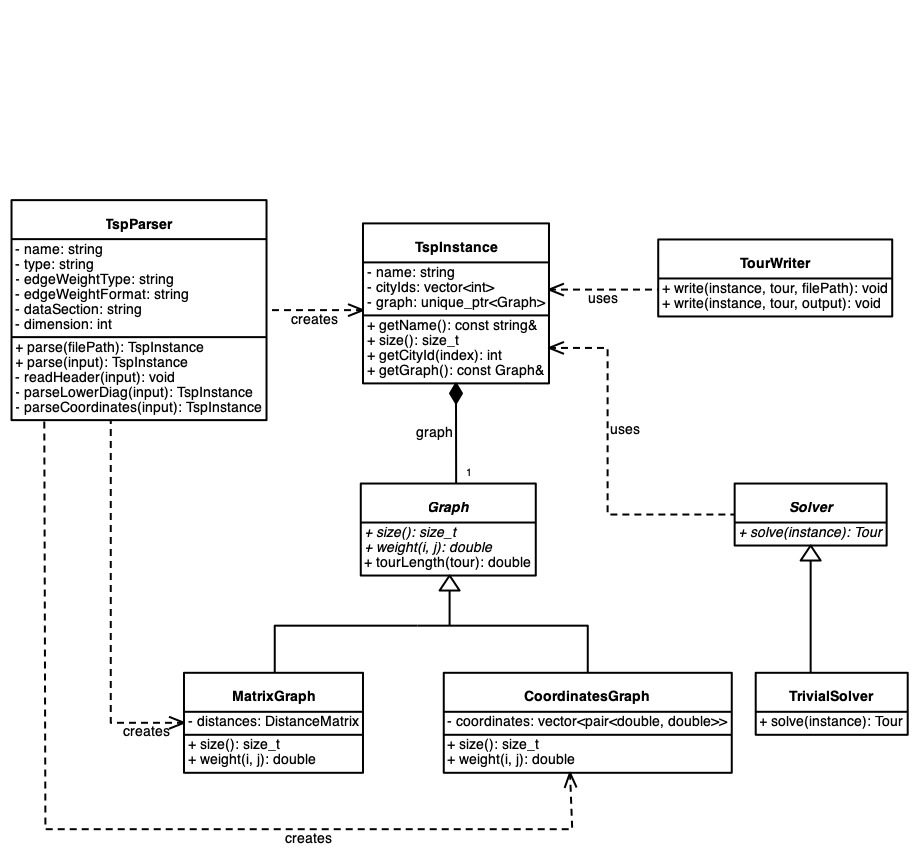
\includegraphics[width=0.95\linewidth,trim=0 0 0 190,clip]{figures/TSP_solver_UML.png}
\caption{Class diagram of the library.}
\label{fig-uml}
\end{figure}

\subsection{Representation of an instance}

An instance combines a name, the identifiers of the cities as written in the file, and a graph. The graph is an abstract class with two operations, which return the number of vertices and the weight of an edge, plus a function that computes the length of a tour. Placing this function in the base class guarantees that every graph and every solver evaluates a tour in the same way.

The matrix graph stores the full symmetric matrix built from the lower triangle. Since the graph is complete, a dense matrix is the natural storage: an adjacency list would hold the same $n(n-1)/2$ edges with slower lookups, while the matrix answers \texttt{weight(i,j)} in constant time. The coordinate graph stores only the points and computes each distance on demand, so its memory grows linearly with the number of cities instead of quadratically. Both classes hide their storage behind the same interface, so a solver is written once for both formats, and both validate their input and indices, so that a defect produces an exception and not undefined behaviour.

Vertices are numbered from zero inside the program. The tour writer is the only place where they are converted back to the identifiers of the file, which keeps off by one errors out of the algorithms.

\subsection{Parsing}\label{sec-parsing}

The parser works in two stages. The header stage reads the \texttt{key : value} lines up to the keyword that opens the data section, and checks that the name, the type and a positive dimension are present. That keyword then selects the data stage, implemented in a separate file for each format. The matrix stage also requires explicit weights in the lower diagonal row format, since other layouts would be read incorrectly. The coordinate stage accepts identifiers starting at 1 (TSPLIB files) or at 0 (course generator) and stores each city at the position given by its identifier.

Besides a file path, the parser accepts any input stream, which lets the tests supply small malformed inputs as strings. Each call resets the state of the parser, so one parser can read several instances. Errors are reported as exceptions whose message names the problem, and only the entry point shows them to the user. We chose exceptions because a parsing failure cannot be corrected locally, and they keep the normal path of the code readable.

The parser is strict about content that changes the meaning of the instance (negative weights, a non zero diagonal, duplicate identifiers, missing or trailing data) and tolerant about the rest, such as spacing around separators, blank lines, Windows line endings and unknown header entries.

\subsection{Solvers}

A solver is any class that implements a common interface with a single function, which takes an instance and returns a tour represented as a vector of vertex indices. The trivial method returns the vertices in increasing order of their index, which is also the order of their identifiers. Because a solver only sees the graph interface and returns a plain vector, it does not depend on the input format or on the output format. Adding a method means adding one class and one line in the function that maps a method name to a solver.

\subsection{Writing tours}

The tour writer converts a tour to the output format. Before writing, it checks that the tour is a permutation of all vertices, so that no solver can produce an output file that violates the specification. The output name is derived from the instance name by replacing a trailing extension, and only a trailing one. A second overload writes to any output stream, which is what the tests use to compare the exact text of the output with the example of the specification. Appendix~\ref{app-tour} shows a complete output file.

\subsection{Entry point and error handling}

The entry point reads the arguments, parses the instance, runs the selected solver and writes the tour. It expects exactly two paths, the instance and the output file, and accepts the option \texttt{-m} followed by a method name anywhere on the command line. Any other option, a missing or extra path, a \texttt{-m} without a value and an unknown method each print a message with the usage and return a non zero status, and the method name is checked before the instance is read. Every error raised by the library, whether in parsing, solving or writing, is an exception derived from the standard exception class. The entry point catches it in one place, prints its message on the error stream and returns the same status. The library classes never print anything themselves, which keeps them reusable and lets the tests check errors without parsing text.

Figure~\ref{fig-flow} shows how these components are connected when the program runs.

\begin{figure}[htbp]
\centering
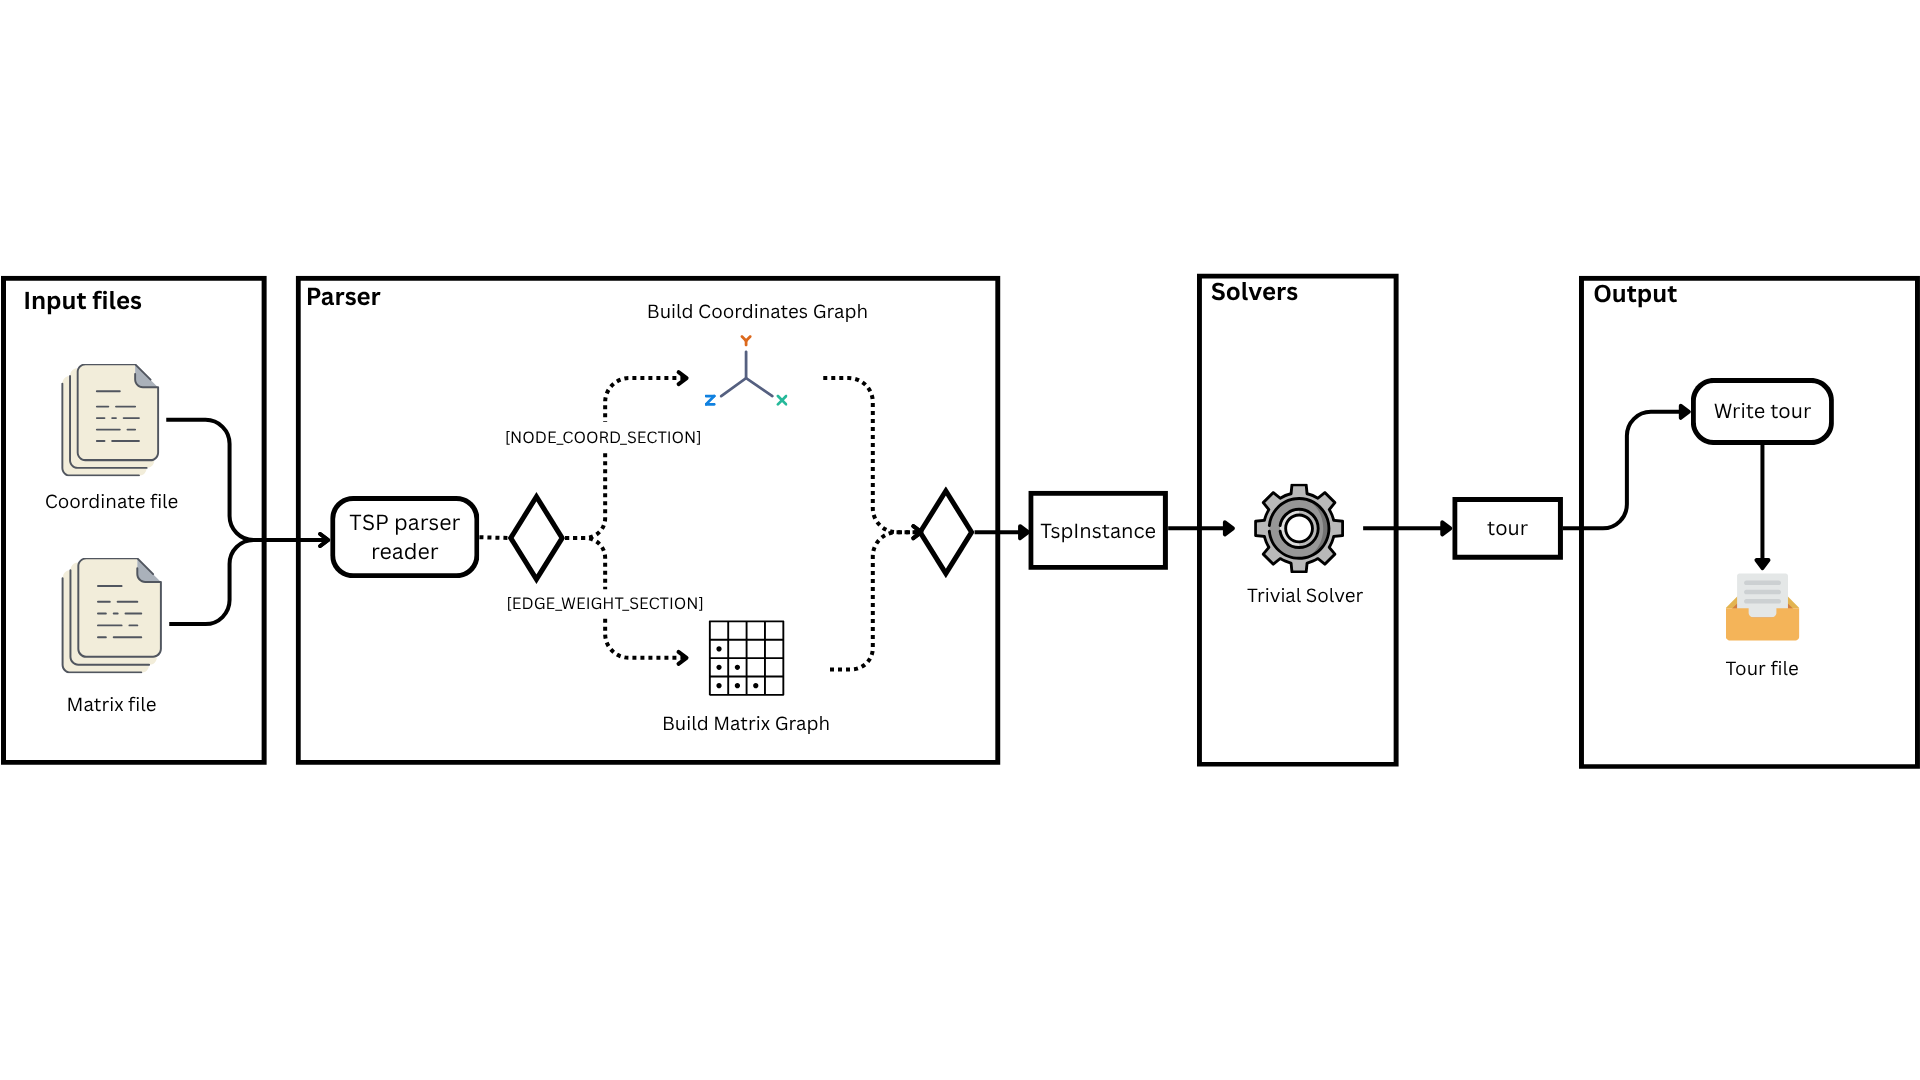
\includegraphics[width=\linewidth,trim=0 225 0 195,clip]{figures/architecture.png}
\caption{Data flow of a run, from the instance file to the tour file.}
\label{fig-flow}
\end{figure}

\section{Key parts of the code}\label{sec-code}

This section shows the short pieces of code that carry the main design decisions. Documentation comments are left out to save space, and some lines are omitted where marked.

\paragraph{The graph interface.} Every solver works only with this abstract class, so it is independent of the file format.
\begin{lstlisting}
class Graph {
    public:
        virtual ~Graph() = default;
        virtual std::size_t size() const = 0;
        virtual double weight(std::size_t i, std::size_t j) const = 0;
        double tourLength(const Tour& tour) const;
};
\end{lstlisting}

\paragraph{Reading the lower triangle.} Weights are read one by one, whatever the line breaks, and each value fills both halves of the symmetric matrix.
\begin{lstlisting}
for (int i = 0; i < dimension; i++) {
    for (int j = 0; j <= i; j++) {
        int weight;
        if (!(input >> weight)) {
            throw std::runtime_error("Missing or invalid integer distance");
        }
        // ... checks for negative weights and a non zero diagonal ...
        distances[i][j] = weight;
        distances[j][i] = weight;
    }
}
\end{lstlisting}

\paragraph{Identifiers starting at 0 or 1.} All lines are read first. The smallest identifier tells whether the file counts from 0 (course generator) or from 1 (TSPLIB), and each city is then stored at the position given by its identifier.
\begin{lstlisting}
const int firstId = (*std::min_element(ids.begin(), ids.end()) == 0) ? 0 : 1;

for (int i = 0; i < dimension; ++i) {
    const int index = ids[i] - firstId;
    if (index < 0 || index >= dimension) {
        throw std::runtime_error("City id out of range");
    }
    if (cityIds[index] != -1) {
        throw std::runtime_error("Duplicate city id");
    }
    cityIds[index] = ids[i];
    coordinates[index] = points[i];
}
\end{lstlisting}

\paragraph{The trivial method.} Since the parsers store the cities in increasing order of their identifiers, visiting the indices in order gives the tour $1 \rightarrow 2 \rightarrow \dots \rightarrow n$.
\begin{lstlisting}
Tour TrivialSolver::solve(const TspInstance& instance) const {
    Tour tour;
    for (std::size_t i = 0; i < instance.size(); i++) {
        tour.push_back(i);
    }
    return tour;
}
\end{lstlisting}

\paragraph{Writing the tour.} The tour is validated before the file is opened, so an invalid tour never empties an existing file.
\begin{lstlisting}
void TourWriter::write(const TspInstance& instance, const Tour& tour,
                       const std::string& filePath) const {
    checkIsPermutation(tour, instance.size());

    std::ofstream output(filePath);
    if (!output.is_open()) {
        throw std::runtime_error("Cannot open output file: " + filePath);
    }
    write(instance, tour, output);
    // ... check that writing succeeded ...
}
\end{lstlisting}

\section{Complexity}\label{sec-complexity}

Table~\ref{tab-complexity} gives the time and memory cost of each component, for an instance with $n$ cities.

\begin{table}[htbp]
\centering\small
\begin{tabularx}{\linewidth}{@{}Y L{3.2cm} L{3.2cm}@{}}
\toprule
Component & Time & Memory \\
\midrule
Reading the header & $O(h)$, $h$ header lines & $O(1)$ \\
Lower diagonal parser (\texttt{MatrixGraph}) & $O(n^2)$ & $O(n^2)$, full matrix \\
Coordinate parser (\texttt{CoordinatesGraph}) & $O(n)$ & $O(n)$, points only \\
\texttt{weight(i,j)} & $O(1)$ & $O(1)$ \\
\texttt{tourLength} & $O(n)$ & $O(1)$ \\
Trivial method & $O(n)$ & $O(n)$ \\
Tour writer, with the permutation check & $O(n)$ & $O(n)$ \\
\midrule
Whole run, matrix file & $O(n^2)$ & $O(n^2)$ \\
Whole run, coordinate file & $O(n)$ & $O(n)$ \\
\midrule
Held-Karp (planned) & $O(n^2 2^n)$ & $O(n 2^n)$ \\
\bottomrule
\end{tabularx}
\caption{Time and memory complexity of each component.}
\label{tab-complexity}
\end{table}

For the trivial method the cost of a run is dominated by reading the file. For a coordinate file the program never builds a matrix, so memory stays linear in the number of cities.

\section{Build and run}\label{sec-run}

The project is built from its root with a single command, which creates \texttt{build/TSPsolver} and \texttt{build/tests}. GoogleTest is downloaded the first time the project is configured.
\begin{lstlisting}[language=bash]
bash build-TSPsolver.sh
\end{lstlisting}

The solver takes the instance path, the output path and an optional method. Without \texttt{-m}, the trivial method is used.
\begin{lstlisting}[language=bash]
./build/TSPsolver TSP-instances/lower_diag/gr17.tsp gr17.tour
./build/TSPsolver TSP-instances/coord/berlin52.tsp berlin52.tour -m trivial
\end{lstlisting}

The tests are run with:
\begin{lstlisting}[language=bash]
./build/tests
\end{lstlisting}

Every invalid use prints a message on the error stream, returns the status 1 and writes no output file. Table~\ref{tab-errors} lists the main cases.

\begin{table}[htbp]
\centering\small
\begin{tabularx}{\linewidth}{@{}L{4.6cm} Y@{}}
\toprule
Situation & Message \\
\midrule
No argument, one path, or an extra path & \texttt{Error: expected an instance path and an output path} \\
\texttt{-m} without a method name & \texttt{Error: -m must be followed by an algorithm name} \\
Unknown option, e.g. \texttt{-x} & \texttt{Error: unknown option \textquotesingle-x\textquotesingle.} \\
Unknown method, e.g. \texttt{-m held-karp} & \texttt{Error: unknown or not yet implemented algorithm \textquotesingle held-karp\textquotesingle.} \\
Instance file not found & \texttt{Error: Cannot open file: <path>} \\
Output folder not found & \texttt{Error: Cannot open output file: <path>} \\
Malformed instance & \texttt{Error:} followed by the reason, e.g. \texttt{Missing NAME} \\
\bottomrule
\end{tabularx}
\caption{Error messages of the command line (exit status 1 in every case).}
\label{tab-errors}
\end{table}

\section{Testing and validation}\label{sec-testing}

\subsection{Unit and executable tests}

The test suite contains 92 tests in 11 groups, and it runs in well under a second. We organised it by component so that a failure points to a single class. Table~\ref{tab-tests} summarises the six test files, and Appendix~\ref{app-tests} lists every test by name.

\begin{table}[htbp]
\centering\small
\begin{tabularx}{\linewidth}{@{}L{3.7cm} c Y@{}}
\toprule
File & Tests & What is checked \\
\midrule
\texttt{ParserTests.cpp} & 32 & Both formats; header variants (spaces around \texttt{:}, Windows line endings, comments); missing or invalid name, type and dimension; truncated and surplus data; duplicate and out of range identifiers; identifiers starting at 0; shuffled lines; negative and non integer weights; wrapped matrix; display section; missing or trailing \texttt{EOF}; real files \\
\texttt{SolverTests.cpp} & 19 & Each of the 15 provided instances is parsed and solved (identifiers, zero diagonal, valid permutation, positive length); sizes of some files; symmetry of \texttt{gr17}; identity tour; single city \\
\texttt{GraphTests.cpp} & 17 & Euclidean distance, symmetry, zero diagonal, triangle inequality, invalid input and indices, tour length including the example of the specification (18), closing edge, independence from start and direction \\
\texttt{ExecutableTests.cpp} & 13 & The real \texttt{TSPsolver}: default and explicit method, \texttt{-m} before or between the paths, unknown method or option, missing method name, extra or missing arguments, missing instance, unwritable output, output read back as a permutation \\
\texttt{TourWriterTests.cpp} & 7 & Exact output of the specification example, tour name, identifiers written instead of indices, invalid tours rejected, file writing, existing file kept on error \\
\texttt{InstanceTests.cpp} & 4 & Getters, missing graph, wrong number of identifiers, out of range identifier \\
\midrule
Total & 92 & \\
\bottomrule
\end{tabularx}
\caption{Content of the test suite.}
\label{tab-tests}
\end{table}

Several tests failed before the corrections described in Section~\ref{sec-process} and now pass, namely the empty matrix, the invalid matrix index, the protection of existing output files, the data after the final keyword in a coordinate file and the identifiers starting at 0. We therefore consider them regression tests for real defects and not only coverage.

\subsection{Instances}

Besides the unit tests, we ran the solver on every provided instance and on generated instances (Table~\ref{tab-instances}). The generated instances, created with \texttt{instance\_generator.py}, number their cities from 0 and range from 1 to 50\,000 cities.

\begin{table}[htbp]
\centering\small
\begin{tabularx}{\linewidth}{@{}L{3.6cm} c Y@{}}
\toprule
Format & Files & Instances \\
\midrule
Lower diagonal matrix & 5 & \texttt{gr17}, \texttt{gr21}, \texttt{gr24}, \texttt{dantzig42}, \texttt{gr48} \\
Coordinates & 10 & \texttt{burma14}, \texttt{ulysses16}, \texttt{att48}, \texttt{berlin52}, \texttt{st70}, \texttt{eil76}, \texttt{pr76}, \texttt{ch130}, \texttt{pr299}, \texttt{pr1002} \\
Generated coordinates & 28 & 1, 5, 20, 100 and 1000 cities (2 files each), and 10, 100, 1000, 5000, 10\,000 and 50\,000 cities (3 files each) \\
\bottomrule
\end{tabularx}
\caption{Instances on which the solver was run.}
\label{tab-instances}
\end{table}

\subsection{Validation with the course checker}

The tour files of the 15 provided instances were submitted to the course solution checker on Moodle, together with their instance file, and all of them were accepted. For example, for \texttt{gr17} the checker reads the instance as an explicit lower triangular matrix of dimension 17, reads our tour $1 \rightarrow 2 \rightarrow \dots \rightarrow 17 \rightarrow 1$ and reports a length of 4722, which is the same value as our own computation. The same check can be run from the command line with the script \texttt{tsp\_check.py}, from the university network or through its VPN.

\section{Performance evaluation}\label{sec-perf}

At this checkpoint only the trivial method exists, so we measure it as the baseline for the methods of the final submission. All times are averages of 5 complete runs (start, reading, solving, writing) on an Apple M5 laptop with 24\,GB of memory, compiled with Apple clang 21 in release mode (\texttt{-O3}).

\paragraph{Solution quality.} Table~\ref{tab-quality} compares the length of the trivial tour with the optimal tour length of each instance. The optimum is not computed by our program: it is the value published with TSPLIB~\cite{tsplib} for each instance. The trivial lengths are computed with the TSPLIB distance functions, as the course checker does (both give 4722 for \texttt{gr17}). The gap is $(\mathrm{trivial} - \mathrm{optimum}) / \mathrm{optimum}$.

\begin{table}[htbp]
\centering\small
\begin{tabular}{@{}l r r r@{\hspace{2.2em}}l r r r@{}}
\toprule
Instance & Trivial & Optimum$^{*}$ & Gap & Instance & Trivial & Optimum$^{*}$ & Gap \\
\midrule
\texttt{burma14} & 4\,562 & 3\,323 & 37\,\% & \texttt{berlin52} & 22\,205 & 7\,542 & 194\,\% \\
\texttt{ulysses16} & 9\,665 & 6\,859 & 41\,\% & \texttt{st70} & 3\,410 & 675 & 405\,\% \\
\texttt{gr17} & 4\,722 & 2\,085 & 126\,\% & \texttt{eil76} & 1\,969 & 538 & 266\,\% \\
\texttt{gr21} & 6\,620 & 2\,707 & 145\,\% & \texttt{pr76} & 150\,781 & 108\,159 & 39\,\% \\
\texttt{gr24} & 3\,436 & 1\,272 & 170\,\% & \texttt{ch130} & 47\,797 & 6\,110 & 682\,\% \\
\texttt{dantzig42} & 699 & 699 & 0\,\% & \texttt{pr299} & 83\,506 & 48\,191 & 73\,\% \\
\texttt{att48} & 49\,840 & 10\,628 & 369\,\% & \texttt{pr1002} & 349\,403 & 259\,045 & 35\,\% \\
\texttt{gr48} & 19\,837 & 5\,046 & 293\,\% & & & & \\
\bottomrule
\end{tabular}
\caption{Length of the trivial tour compared with the optimal tour length. $^{*}$Published with TSPLIB, not computed by our program.}
\label{tab-quality}
\end{table}

The trivial tour is 35\,\% to 682\,\% longer than the optimum, depending only on how the cities happen to be numbered in each file. The one exception, \texttt{dantzig42}, lists its cities in the order of an optimal tour. These values are the reference that the next methods must improve on, and the Held-Karp algorithm will have to reach the published optimum exactly on the small instances.

\paragraph{Time and scalability.} The 15 provided instances all run in 1.8 to 8.7\,ms (\texttt{pr1002} is the slowest). Table~\ref{tab-time} shows generated instances of increasing size, three per size.

\begin{table}[htbp]
\centering\small
\begin{tabular}{@{}l r r r r r r@{}}
\toprule
Cities $n$ & 10 & 100 & 1\,000 & 5\,000 & 10\,000 & 50\,000 \\
Time (ms) & 2.1 & 1.9 & 2.9 & 4.3 & 10.7 & 17.1 \\
\bottomrule
\end{tabular}
\caption{Average time of a complete run on generated instances.}
\label{tab-time}
\end{table}

Up to about a thousand cities the time is dominated by a fixed cost of about 2\,ms for starting the program, so it hardly depends on $n$. Beyond that it grows with $n$, as expected from the linear cost of reading and writing the cities (Section~\ref{sec-complexity}). At this scale the measurements are noisy, so they give orders of magnitude only. The cost of the solving step itself will matter with the Held-Karp algorithm, whose time grows exponentially.

\section{Specification compliance}\label{sec-compliance}

Table~\ref{tab-compliance} lists the requirements of the subject~\cite{subject} and where they are met.

\begin{table}[htbp]
\centering\small
\begin{tabularx}{\linewidth}{@{}l Y l l@{}}
\toprule
Spec. & Requirement & Status & Where \\
\midrule
2.1.1 & \texttt{bash build-TSPsolver.sh} at the root builds the project & Done & Section~\ref{sec-run} \\
2.1.1 & \texttt{build/TSPsolver} and \texttt{build/tests} are created & Done & Section~\ref{sec-run} \\
2.1.2 & \texttt{TSPsolver <instance> <output>} runs the default method & Done & Section~\ref{sec-run} \\
2.1.3 & \texttt{-m trivial} & Done & Section~\ref{sec-run} \\
2.1.3 & \texttt{-m held-karp} and a third method & Final submission & Section~\ref{sec-future} \\
2.1.4 & \texttt{./build/tests} runs all the tests & Done (92 tests) & Section~\ref{sec-testing} \\
2.2 & Coordinate files (\texttt{NODE\_COORD\_SECTION}) & Done (10 files) & Table~\ref{tab-instances} \\
2.2 & Lower diagonal files (\texttt{LOWER\_DIAG\_ROW}) & Done (5 files) & Table~\ref{tab-instances} \\
2.3 & Tour file format & Done, accepted by the checker & Section~\ref{sec-testing} \\
2.4.1 & Trivial method & Done & Section~\ref{sec-code} \\
2.4.2 & Held-Karp algorithm & Final submission & Section~\ref{sec-future} \\
2.5 & Performance evaluation & Baseline done & Section~\ref{sec-perf} \\
3 & Mid-term version supporting the trivial method & Done & This report \\
3.2 & Report as a PDF document & Done & This report \\
\bottomrule
\end{tabularx}
\caption{Requirements of the subject and their status at the checkpoint.}
\label{tab-compliance}
\end{table}

\section{Limitations and decisions}\label{sec-limits}

The subject leaves some points open. Table~\ref{tab-decisions} lists the decisions we took.

\begin{table}[htbp]
\centering\small
\begin{tabularx}{\linewidth}{@{}L{4.6cm} Y@{}}
\toprule
Point & Decision \\
\midrule
\texttt{EOF} keyword & Optional, since \texttt{pr1002} has none; any data after it is rejected \\
\texttt{DISPLAY\_DATA\_SECTION} & Skipped, since it only holds drawing coordinates (\texttt{dantzig42}) \\
City identifiers & May start at 1 (TSPLIB) or at 0 (course generator); the tour file uses the identifiers of the input \\
\texttt{NAME} of the tour file & Instance name with a trailing \texttt{.tsp} removed, followed by \texttt{.tour} \\
Default method & Trivial \\
Command line & Exactly two paths, \texttt{-m} anywhere, any other argument rejected \\
Distances of coordinate files & Plain Euclidean distance, whatever \texttt{EDGE\_WEIGHT\_TYPE} says \\
\bottomrule
\end{tabularx}
\caption{Decisions on points left open by the subject.}
\label{tab-decisions}
\end{table}

The main limitation is the last decision. TSPLIB defines several distance functions: rounded Euclidean (\texttt{EUC\_2D}), geographical (\texttt{GEO}) and pseudo Euclidean (\texttt{ATT}). Our coordinate graph uses the plain Euclidean distance without rounding for every file. The tours we write are not affected, since the trivial method does not use distances, but the lengths our program would compute differ from the official ones. The difference is small for \texttt{EUC\_2D} files (\texttt{eil76}: 1974.7 instead of 1969), but large for the other types, because \texttt{GEO} coordinates are latitudes and longitudes and \texttt{ATT} uses a scaled distance (\texttt{burma14}: 42.5 instead of 4562; \texttt{att48}: 157\,530 instead of 49\,840). This must be fixed before comparing the lengths of the next methods with the published optima.

The second limitation is that the trivial method makes no attempt to produce a short tour, since its purpose is to validate the pipeline from parsing to output (Table~\ref{tab-quality}).

\section{Future work}\label{sec-future}

For the final submission we plan the following steps, in this order.
\begin{enumerate}
  \item \textbf{TSPLIB distances.} Read \texttt{EDGE\_WEIGHT\_TYPE} and give the coordinate graph the matching distance function (\texttt{EUC\_2D}, \texttt{GEO}, \texttt{ATT}), and check the lengths against the course checker.
  \item \textbf{Held-Karp algorithm}~\cite{heldkarp}. Dynamic programming over subsets with a bitmask, plus backtracking to recover the tour. Its table needs $n \cdot 2^{n-1}$ values, about 84\,MB for $n = 20$ and 3.4\,GB for $n = 25$, so the solver will refuse instances above a size limit instead of running out of memory. It must give the known optima, for example 2085 on \texttt{gr17} and 3323 on \texttt{burma14}.
  \item \textbf{Third method.} A heuristic for large instances, for example a nearest neighbour tour improved by 2-opt, to be discussed with the teacher before coding.
  \item \textbf{Measurements.} Time the solving step alone inside the program, print the tour length, and repeat Section~\ref{sec-perf} for the three methods.
\end{enumerate}

\section{Reflections}

The most useful decision of the first weeks was to fix the structure of the code early. It allowed us to add the second input format in three small commits without touching existing code. The review of 14 October was less comfortable, since it showed that several parts we considered complete had behaviour that we had never exercised. The problems with the output file and the matrix accessor would not have appeared in normal use, and we only found them because the tests supplied inputs that a careful user would not. If we repeated the project, we would write the tests of each component at the same time as the component.

Two further lessons came from the last days before the checkpoint. First, a program that works on our machines is not enough: the build has to be checked exactly as the grader will run it, from a clean copy and with the commands of the subject, which is how we found that the executable had the wrong name and location. Second, working on two separate branches for two weeks made the final merge harder than it needed to be. Agreeing on the shared classes first helped, but merging more often would have shown integration problems earlier.

\section{Use of AI tools}


\begin{thebibliography}{9}
\bibitem{subject} E.~Foussard. \emph{Project -- Solving the Travelling Salesman Problem}. Programming course, M1 AI, Universit\'e Grenoble Alpes, 2026.
\bibitem{tp4} E.~Foussard. \emph{TP4 -- Object-Oriented Programming and Graphs}. Programming course, M1 AI, Universit\'e Grenoble Alpes, 2026.
\bibitem{tsplib} G.~Reinelt. \emph{TSPLIB 95}. Universit\"at Heidelberg, 1995. Optimal tour lengths, archived copy: \url{https://web.archive.org/web/20231203135812/http://comopt.ifi.uni-heidelberg.de/software/TSPLIB95/STSP.html}
\bibitem{heldkarp} M.~Held and R.~M.~Karp. A dynamic programming approach to sequencing problems. \emph{Journal of the Society for Industrial and Applied Mathematics}, 10(1):196--210, 1962.
\bibitem{gtest} Google. \emph{GoogleTest}, version 1.17.0. \url{https://github.com/google/googletest}
\end{thebibliography}

\clearpage
\appendix

\section{Example of an output file}\label{app-tour}

Tour file written by \texttt{./build/TSPsolver TSP-instances/lower\_diag/gr17.tsp gr17.tour}. The lines for cities 4 to 14 are left out.

\noindent\begin{minipage}{\linewidth}
\begin{lstlisting}[language={}]
NAME : gr17.tour
TYPE : TOUR
DIMENSION : 17
TOUR_SECTION
1
2
3
...
15
16
17
-1
EOF
\end{lstlisting}
\end{minipage}

\section{List of tests}\label{app-tests}

The 92 tests of \texttt{./build/tests}, grouped by file. \texttt{ParseAndTrivialSolve} runs once for each of the 15 provided instances.

{\scriptsize
\begin{multicols}{2}
\raggedright
\textbf{ParserTests.cpp (32)}\\
\texttt{ReadsCoordinateInstance}, \texttt{ReadsLowerDiagInstance}, \texttt{AcceptsSpaceBeforeColonAndWindowsLineEndings}, \texttt{IgnoresCommentsAndUnknownHeaderEntries}, \texttt{AcceptsMissingFinalEof}, \texttt{AcceptsScientificNotationAndNegativeCoordinates}, \texttt{StoresCoordinatesByIdWhenLinesAreShuffled}, \texttt{SkipsDisplayDataSectionAfterMatrix}, \texttt{ParserCanBeReusedAcrossInstances}, \texttt{RejectsMissingFile}, \texttt{RejectsEmptyInput}, \texttt{RejectsMissingName}, \texttt{RejectsWrongType}, \texttt{RejectsMissingOrInvalidDimension}, \texttt{RejectsHeaderLineWithoutColon}, \texttt{RejectsMissingDataSection}, \texttt{RejectsTruncatedCoordinates}, \texttt{RejectsNonNumericCoordinate}, \texttt{RejectsOutOfRangeAndDuplicateCityIds}, \texttt{AcceptsIdsStartingAtZeroLikeTheInstanceGenerator}, \texttt{StoresZeroBasedIdsByIdWhenLinesAreShuffled}, \texttt{RejectsExtraCoordinateLines}, \texttt{RejectsMatrixWithWrongFormat}, \texttt{RejectsInvalidMatrixValues}, \texttt{RejectsTrailingDataAfterMatrix}, \texttt{AcceptsMatrixWithoutFinalEof}, \texttt{AcceptsMatrixWrappedOverArbitraryLines}, \texttt{IgnoresBlankLinesAndIndentationInHeaderAndData}, \texttt{RejectsUnexpectedDataAfterCoordinates}, \texttt{RejectsMatrixShorterThanDimension}, \texttt{RejectsNonIntegerMatrixWeight}, \texttt{ParsesEveryProvidedInstanceWithItsDeclaredDimension}

\medskip
\textbf{SolverTests.cpp (19)}\\
\texttt{ParseAndTrivialSolve} (15 instances), \texttt{MatchTheirNames}, \texttt{Gr17MatrixIsSymmetric}, \texttt{ReturnsIdentityPermutation}, \texttt{HandlesSingleCity}

\columnbreak
\textbf{GraphTests.cpp (17)}\\
\texttt{ComputesEuclideanDistance}, \texttt{IsSymmetricWithZeroDiagonal}, \texttt{SatisfiesTriangleInequality}, \texttt{RejectsEmptyInput}, \texttt{RejectsOutOfRangeIndex} (coordinates), \texttt{ReturnsStoredWeights}, \texttt{RejectsNonSquareMatrix}, \texttt{RejectsEmptyMatrix}, \texttt{RejectsOutOfRangeIndex} (matrix), \texttt{MatchesSpecificationExample}, \texttt{ClosesTheCycle}, \texttt{IsIndependentOfStartAndDirection}, \texttt{SingleCityAndEmptyTourHaveZeroLength}, \texttt{RejectsInvalidVertex}, \texttt{ChecksEveryVertexNotOnlyTheFirstOne}, \texttt{PrefersPerimeterOrderOnASquare}, \texttt{CoincidentCitiesAreAtDistanceZero}

\medskip
\textbf{ExecutableTests.cpp (13)}\\
\texttt{SolvesWithDefaultMethod}, \texttt{AcceptsExplicitTrivialMethod}, \texttt{FailsOnUnknownAlgorithmWithoutWritingOutput}, \texttt{FailsOnMissingInstance}, \texttt{FailsWithoutArguments}, \texttt{AcceptsMethodBeforeThePaths}, \texttt{AcceptsMethodBetweenThePaths}, \texttt{FailsWhenMethodNameIsMissing}, \texttt{FailsOnUnknownOption}, \texttt{FailsOnExtraArgument}, \texttt{FailsWithOnlyOneArgument}, \texttt{FailsOnUnwritableOutput}, \texttt{OutputCanBeReadBackAsAPermutation}

\medskip
\textbf{TourWriterTests.cpp (7)}\\
\texttt{WritesSpecificationFormat}, \texttt{OnlyReplacesTspExtensionAtTheEnd}, \texttt{OutputsCityIdsNotIndices}, \texttt{RejectsInvalidTours}, \texttt{WritesFile}, \texttt{FailsOnUnwritablePath}, \texttt{InvalidTourDoesNotTouchExistingFile}

\medskip
\textbf{InstanceTests.cpp (4)}\\
\texttt{ExposesNameSizeAndIds}, \texttt{RejectsMissingGraph}, \texttt{RejectsIdCountMismatch}, \texttt{RejectsOutOfRangeCityId}
\end{multicols}
}

\end{document}
